% -*- latex -*-
%%%%%%%%%%%%%%%%%%%%%%%%%%%%%%%%%%%%%%%%%%%%%%%%%%%%%%%%%%%%%%%%
%%%%%%%%%%%%%%%%%%%%%%%%%%%%%%%%%%%%%%%%%%%%%%%%%%%%%%%%%%%%%%%%
%%%%
%%%% This text file is part of the source of 
%%%% 'Parallel techniques'
%%%% by Ángel de Vicente, copyright 2019
%%%%
%%%% TO DO:
%%%%
%%%% mpi-slides.tex : introduction to MPI concepts
%%%%      Slides adapted from
%%%%       https://doc.itc.rwth-aachen.de/display/VE/PPCES+2016
%%%%
%%%%%%%%%%%%%%%%%%%%%%%%%%%%%%%%%%%%%%%%%%%%%%%%%%%%%%%%%%%%%%%%
%%%%%%%%%%%%%%%%%%%%%%%%%%%%%%%%%%%%%%%%%%%%%%%%%%%%%%%%%%%%%%%%

In order to improve the performance of the Barnes-Hut algorithm learned in the
previous chapter, we will now learn about parallel programming, so several
computers can collaborate to complete the same problem.


\Level 0 {Basic MPI}
\label{sec:basic-mpi}

%\includepdf[frame=true,scale=0.98,pages={2-12,18-19}]{graphics/01_PPCES2016_MPI_Tutorial.pdf}
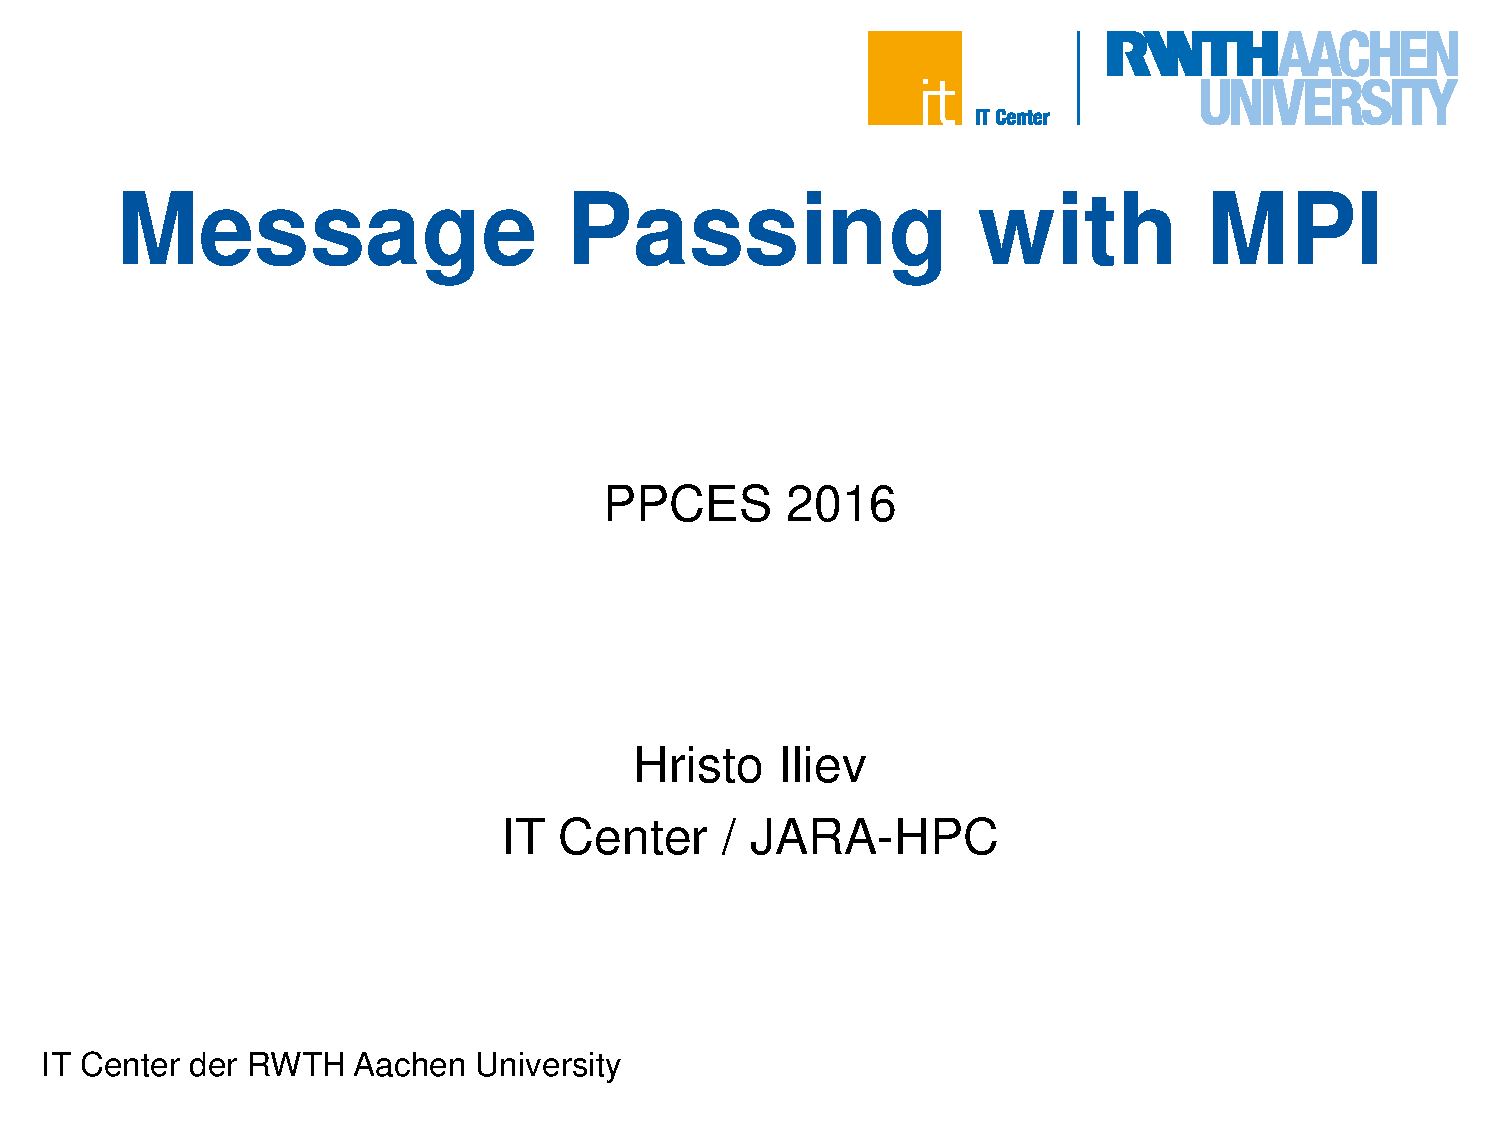
\includepdf[frame=true,scale=0.98,pages={1,4-6,9-12,14-16,19-22,26,27-34,37-41,43-44,46-47,50}]{graphics/01_PPCES2016_MPI_Tutorial.pdf}
%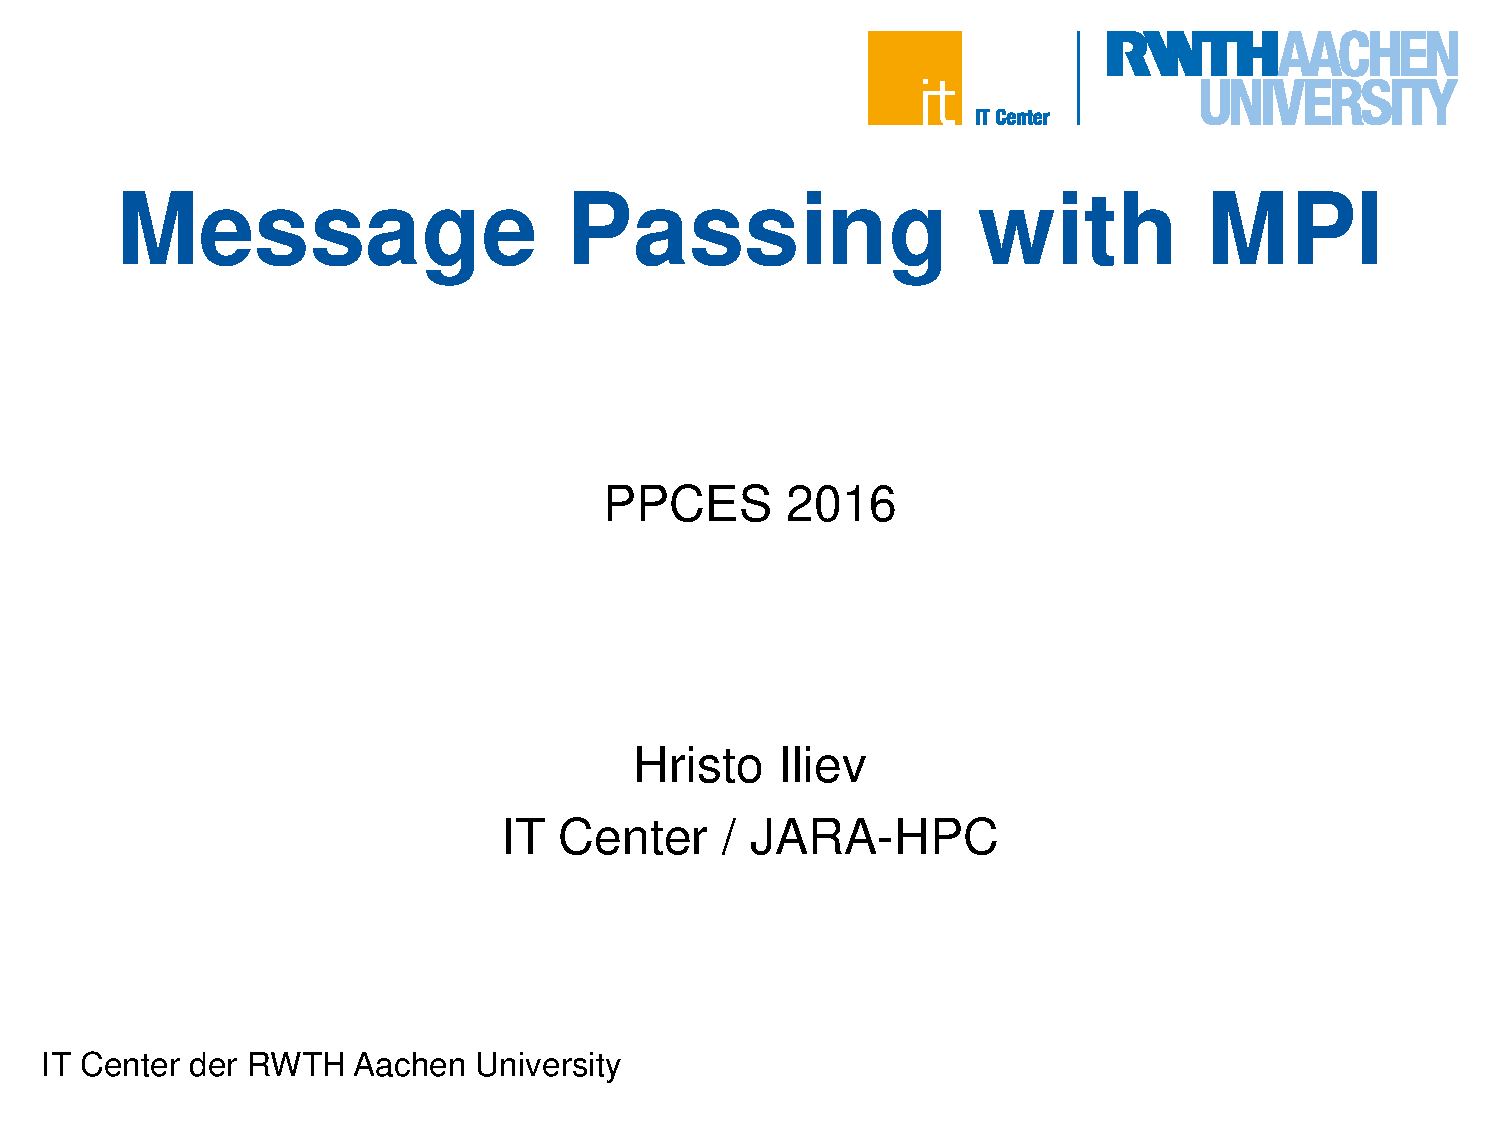
\includepdf[frame=true,scale=0.98,pages={1-}]{graphics/02_PPCES2016_MPI_Tutorial.pdf}
%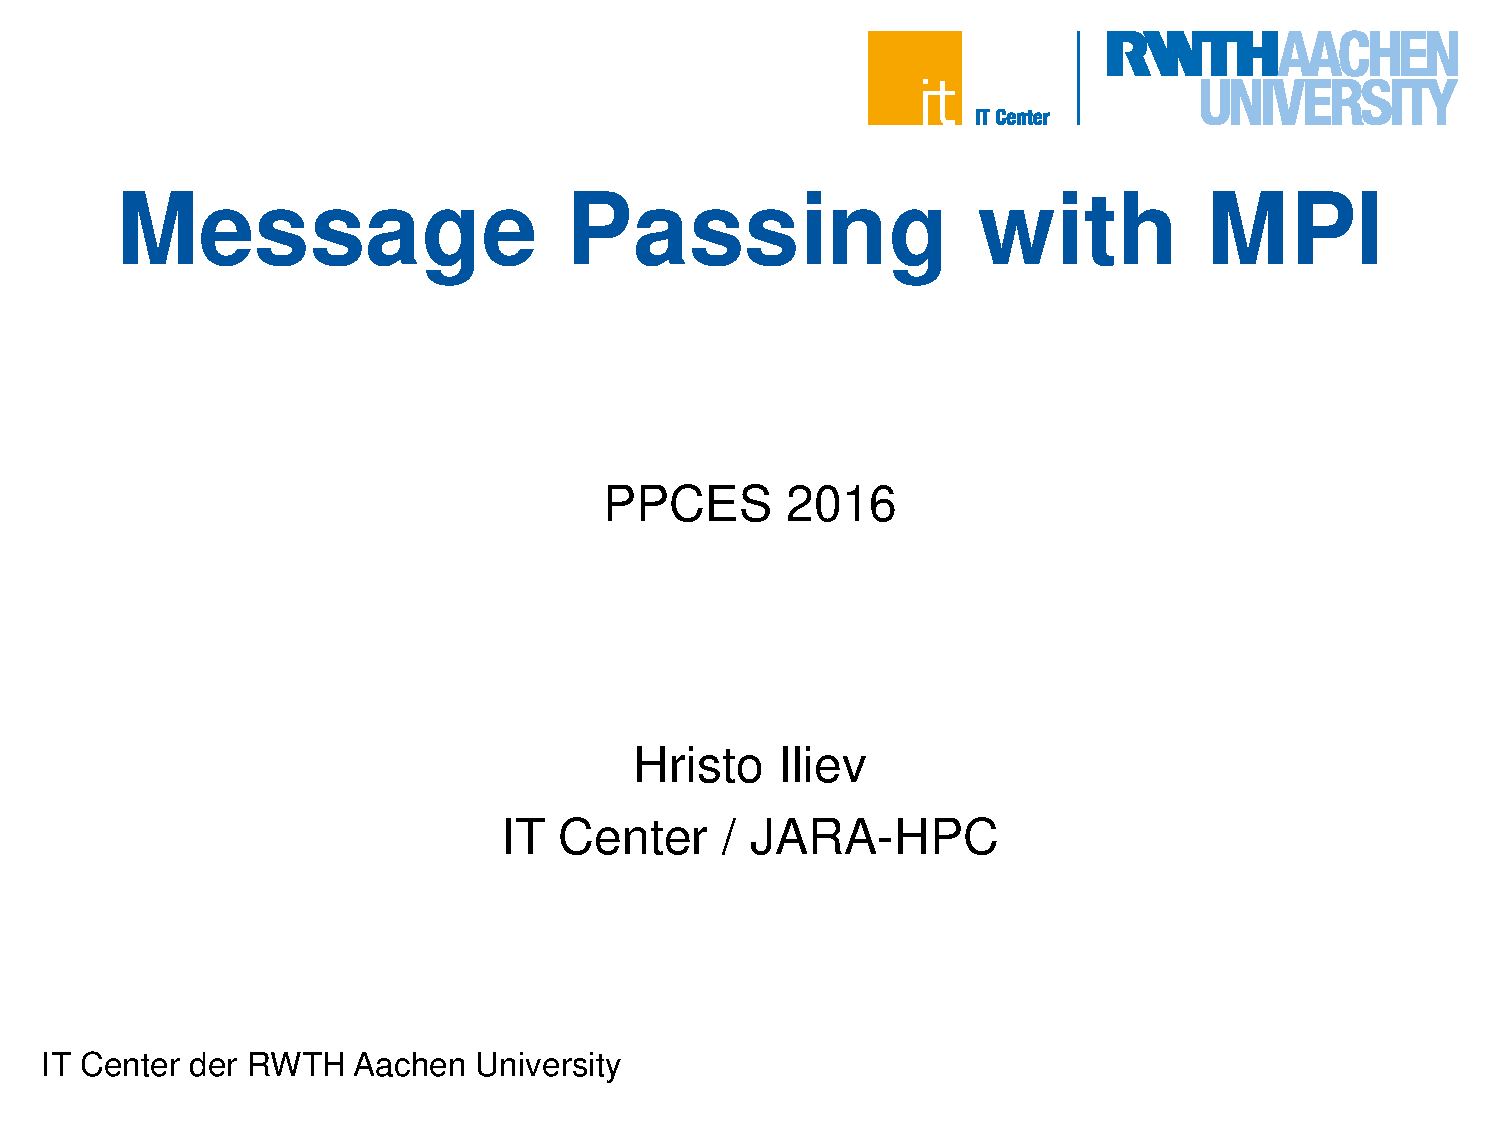
\includepdf[frame=true,scale=0.98,pages={1-}]{graphics/03_PPCES2016_MPI_Tutorial.pdf}

\Level 1 {MPI parallel programs in the CCA}
To run a basic parallel ``Hello World!'' program in the CCA machines, you would
need to follow these steps:

\begin{enumerate}

\item Write the hello-world.f90 code:

\begin{verbatim}

program hello_world
  use mpi
  implicit none

  integer error
  integer, parameter :: master = 0
  integer num_procs
  integer world_id

  call MPI_Init ( error )
  call MPI_Comm_size ( MPI_COMM_WORLD, num_procs, error )
  call MPI_Comm_rank ( MPI_COMM_WORLD, world_id, error )

  if ( world_id == master ) then
     print*, "I'm the master of ", num_procs, "processes"
  end if

  print*, "Process ", world_id, ' says "Hello, world!"'

  call MPI_Finalize ( error )

end program hello_world
\end{verbatim}

\item Compile it using the mpif90 wrapper

\begin{verbatim}  

[angelv@opel]$ mpif90 -o hello-world hello-world.f90
\end{verbatim}

\item Then you just execute it, selecting the number of processes to create with
  the -np option

\begin{verbatim}

[angelv@opel]$ mpirun -np 4 ./hello-world
I'm the master of            4 processes
Process            0  says "Hello, world!"
Process            1  says "Hello, world!"
Process            2  says "Hello, world!"
Process            3  says "Hello, world!"
[angelv@opel]$
\end{verbatim}

\end{enumerate}

\includepdf[frame=true,scale=0.98,pages={26}]{graphics/mpi_part1.pdf}
\includepdf[frame=true,scale=0.98,pages={53-54,56-60,63,85}]{graphics/01_PPCES2016_MPI_Tutorial.pdf}

\includepdf[frame=true,scale=0.98,pages={42}]{graphics/mpi_part1.pdf}

\Level 1 {MPI Parallel code to calculate an integral using the trapezoidal rule}
\label{sec:trapezoidal-rule}

\begin{verbatim}
!  trap.f -- Parallel Trapezoidal Rule, first version
!
! Slightly modified by Angel de Vicente
!
!  Input: None.
!  Output:  Estimate of the integral from a to b of f(x) 
!     using the trapezoidal rule and n trapezoids.
! 
!  Algorithm:
!     1.  Each process calculates "its" interval of 
!         integration.
!     2.  Each process estimates the integral of f(x)
!         over its interval using the trapezoidal rule.
!     3a. Each process != 0 sends its integral to 0.
!     3b. Process 0 sums the calculations received from
!         the individual processes and prints the result.
! 
!  Notes:  
!     1.  f(x), a, b, and n are all hardwired.
!     2.  Assumes number of processes (p) evenly divides
!         number of trapezoids (n = 1024)
!
! See section 3.2 de "MPI User's Guide in Fortran"
!
PROGRAM trapezoidal
  USE MPI
  INTEGER :: n=1024, dest=0, tag=0
  REAL :: a=0.0, b=1.0
  INTEGER :: my_rank, p, local_n, source, status(MPI_STATUS_SIZE), ierr
  REAL :: h, local_a, local_b, integral, total
  
  call MPI_INIT(ierr)
  call MPI_COMM_RANK(MPI_COMM_WORLD, my_rank, ierr)
  call MPI_COMM_SIZE(MPI_COMM_WORLD, p, ierr)
	
  h = (b-a)/n
  local_n = n/p
	
  local_a = a + my_rank*local_n*h
  local_b = local_a + local_n*h
  integral = Trap(local_a, local_b, local_n, h)
	
  IF (my_rank .EQ. 0) THEN
     total = integral
     DO source = 1, p-1
        CALL MPI_RECV(integral, 1, MPI_REAL, source, tag, MPI_COMM_WORLD, status, ierr)
        total = total + integral
     END DO
  ELSE
     CALL MPI_SEND(integral, 1, MPI_REAL, dest, tag, MPI_COMM_WORLD, ierr)
  END IF
	
  IF (my_rank .EQ. 0) THEN
     PRINT*, "With n = ", n, " trapezoids, our estimate"
     PRINT*, "of the integral from ", a, " to ", b, " = ", total
  END IF

  CALL MPI_FINALIZE(ierr) 

CONTAINS
  REAL FUNCTION f(x)
    REAL :: x

    f = x*x
  END FUNCTION f


  REAL FUNCTION Trap(local_a, local_b, local_n, h)
    REAL ::   local_a, local_b, h, integral, x, i
    INTEGER :: local_n

    integral = (f(local_a) + f(local_b))/2.0 
    x = local_a 
    DO i = 1, local_n-1
       x = x + h 
       integral = integral + f(x) 
    END DO
    Trap = integral*h 
  END FUNCTION Trap

END PROGRAM trapezoidal
\end{verbatim}
  
\Level 0 {Basic MPI Exercises - Point-to-Point}
\label{sec:basic-mpi-exercises}

Below there are some exercises to familiarize yourself with the basic features
of MPI, using the most basic point-to-point routines (those in which only two
processes take part in the communication), as seen in section
\ref{sec:basic-mpi}.

You can find solutions to these exercises in section
\ref{app:sol-basic-mpi}, but you are \emph{highly encouraged} to try to solve
them first on your own.

\Level 1 {Simple modification to ``Hello World!''}
\label{ex:basic-mpi-modified-hello}

In this exercise, we will make a simple modification to the "Hello World!"
problem. 

In this case, we want that each process with rank$>$0 sends a message to the
process with rank==0. The message is just its rank, and process 0 will just
print a message saying that it received the message. (You will have to use the
routines MPI\_Send and MPI\_Recv).

Thus, for example, if we run the code with 4 processes, we could get the
following output: 

\begin{verbatim}
Greetings from process 1 !
Greetings from process 2 !
Greetings from process 3 !
\end{verbatim}

Remember that the code is meant to run with any number of processes, not only
4. Also, make sure you understand if the messages should be printed in
consecutive order or not, and in any case why.

\Level 1 {Ring data passing}
\label{ex:basic-mpi-ring}

Write a parallel program (valid for any number N of processes), in which:

\begin{itemize}
\item rank 0 reads a number

\item each process with rank==r sends to the process with rank==r+1 the number
received (read in the case of rank=0) multiplied by r+1, except the last process
(rank==N-1), who sends is to the process with rank=0

\item rank 0 prints the number that it receives from process with rank==N-1

\end{itemize}

\Level 1 {Parallel sum}
\label{ex:basic-mpi-sum}

Write a parallel program to compute the sum of a 1-D array:

\begin{itemize}
\item rank 0 reads the array 1-D array size

\item rank 0 allocates an array with the given size and reads the data

\item rank 0 calculates the number of data that each rank will be responsible for
(we can assume that the array size is divisible by the number of processes running
the code)

\item rank 0 sends to each process the number of items it will responsible for and
the actual data (which each process will have to store in an temporary array,
              
\item each process will calculate the partial sum of its array chunk and will send
the partial result to rank 0

\item rank 0 will calculate the total sum and print the result.

\end{itemize}


\Level 1 {Matrix distribution}
\label{ex:basic-mpi-matrix-distribution}

This exercise was taken from the "Training MPI" course by CINECA-SCAI. For
details see \url{http://www.hpc.cineca.it/content/exercise-5}

Distribute a global square NxN matrix (with N fixed) over P processors, so that
each task has a local portion of it in its memory. Initialize such portion with
the task's rank.

\textit{NOTE: the exercise does not state that P has to be a divisor of N. How to deal
with the matrix distribution if the number of rows/columns isn't the same for
all tasks?}

Each task sends its first and last columns (if Fortran) or rows (if C) to its
neighbours (i.e.: the first column/row to the left processor, the last
column/row to the right processor). Note that each task has to actually allocate
a larger portion of its submatrix (ghost cells), with two extra columns/rows at
the extremities to hold the received values.  

\Level 1 {Identity matrix distribution}
\label{ex:basic-mpi-id-matrix-distribution}

This exercise was taken from the "Training MPI" course by CINECA-SCAI. For
details see \url{http://www.hpc.cineca.it/content/exercise-6}

Write a program that performs a data distribution over the processes of the
identity matrix. Given the number of processes and the dimension of the identity
matrix, each process must allocate its own portion of the matrix. Distribute the
matrix by columns (FORTRAN).

First, obtain the number, N,  of columns you need to allocate for each
process, np. In case N is not divisible by np, take care of the remainder with
the module operator (function).

Now you need to implement a transformation from global to local (task)
coordinates. You can use a a varable, iglob, that shifts the values to be
initialized to 1 according to the global coordinates.

To check if everything is correct make the process 0 collect all matrix blocks
initialized by the other processes and print out the matrix.

